\subsection{$|d_{0}^{\textrm{sig}}|$ selection efficiency for fake and real leptons}
\label{app:boosted_fakelepton_d0eff}

In this appendix, the efficiency of the lepton impact parameter significance ($|d_{0}^{\textrm{sig}}|$) selection on real and fake
leptons is evaluated in MC samples. The Pythia 8 dijet sample is used as a source for fake and non-prompt leptons and the W+jets, 
non-resonant SM di-Higgs and resonant scalar with $m_{H} = 1500 \GeV$ samples are used as sources for real leptons. 
For all MC samples, the efficiency of the $|d_{0}^{\textrm{sig}}|$ selection is evaluated after the event reconstruction level 
(Sec~\ref{sec:boosted_evtreco}) but without any event selection applied described in Section~\ref{sec:boosted_evtsel} and 
\ref{sec:boosted_regiondefs}. The looser criteria with respect to the final selection level in the analysis is needed to retain 
reasonable statistics for the dijet sample.

Table~\ref{tab:boosted_fakelepton_d0sigcuteff} shows the fraction of events (in percent) passing or failing the 
lepton $|d_{0}^{\textrm{sig}}|$ selection for different MC samples. Events with lepton $|d_{0}^{\textrm{sig}}|$ < 2.0 
are considered as s\textit{pass} and $|d_{0}^{\textrm{sig}}|$ > 2.0 are considered as \textit{fail}. 


\begin{table}[!htbp]
\begin{center}
\begin{tabular}{|c|c|c|c|c|}

\multirow{2}{*}{Samples} & \multicolumn{2}{c|}{Electrons} & \multicolumn{2}{c|}{Muons} \\
\cline{2-5}
&  Pass & Fail & Pass & Fail \\
\hline
Dijet   (Fake) &  84.6 $\pm$ 3.4 & 15.4 $\pm$ 3.4  & 62.3 $\pm$ 8.3 & 37.7 $\pm$ 8.3 \\
W+jets  (Real) &  92.9 $\pm$ 0.1 & 7.2  $\pm$ 0.1  & 93.6 $\pm$ 0.0 & 6.4  $\pm$ 0.0 \\
SMhh    (Real) &  92.4 $\pm$ 1.3 & 7.6  $\pm$ 1.3  & 90.4 $\pm$ 2.2 & 9.6  $\pm$ 2.2 \\
Xhh1500 (Real) &  93.3 $\pm$ 0.3 & 6.7  $\pm$ 0.3  & 93.4 $\pm$ 0.3 & 6.6  $\pm$ 0.3 \\
\end{tabular}
\end{center}
\caption{The fraction of events (in percent) passing or failing the lepton impact parameter 
significance ($|d_{0}^{\textrm{sig}}|$) selection for different MC samples. The dijet sample
is used as the source for fake and non-prompt leptons while the W+jets, SMhh and Xhh1500
samples are used as sources for real leptons.
} 
\label{tab:boosted_fakelepton_d0sigcuteff}
\end{table}


\subsection{Fake lepton origin composition in dijet MC}
\label{app:boosted_fakelepton_composition}

\newcommand{\OriginFootnote}{%
The number code labelling each classified origin is documented as "ParticleOrigin" enumerated type 
in the~\href{https://svnweb.cern.ch/cern/wsvn/atlasoff/PhysicsAnalysis/MCTruthClassifier/trunk/MCTruthClassifier/MCTruthClassifierDefs.h}
{MCTruthClassifierDefs.h} header file within the \texttt{MCTruthClassifier} package.}

The origin of the fake leptons and their compsition is evaluated using the dijet MC sample. The origin
of each reconstructed lepton is classified by the \apkg{https://twiki.cern.ch/twiki/bin/view/AtlasProtected/MCTruthClassifier}
{MCTruthClassifier} package. The package assigns an integer number code label\footnote{\OriginFootnote} for all reconstructed 
leptons which corresponds to a truth-level classification of the origin of the lepton. The origin number codes related to this study is 
listed in Table~\ref{tab:boosted_fakeorigin_origincode}.



\begin{table}[!htbp]
\begin{center}
\begin{tabular}{|c|c|}

Origin        &  \texttt{MCTruthClassifier} code \\
\hline
NonDefined    & 0  \\
PhotonConv    & 5  \\
DalitzDec     & 6  \\
TauLep        & 9  \\
LightMeson    & 23 \\
StrangeMeson  & 24 \\
CharmedMeson  & 25 \\
BottomMeson   & 26 \\
LightBaryon   & 30 \\
StrangeBaryon & 31 \\
CharmedBaryon & 32 \\
BottomBaryon  & 33 \\
PionDecay     & 34 \\
KaonDecay     & 35 \\
\end{tabular}
\end{center}
\caption{\texttt{MCTruthClassifier} code designated origin for reconstructed leptons.}
\label{tab:boosted_fakeorigin_origincode}
\end{table}

\begin{figure}[!htbp]
\begin{center}

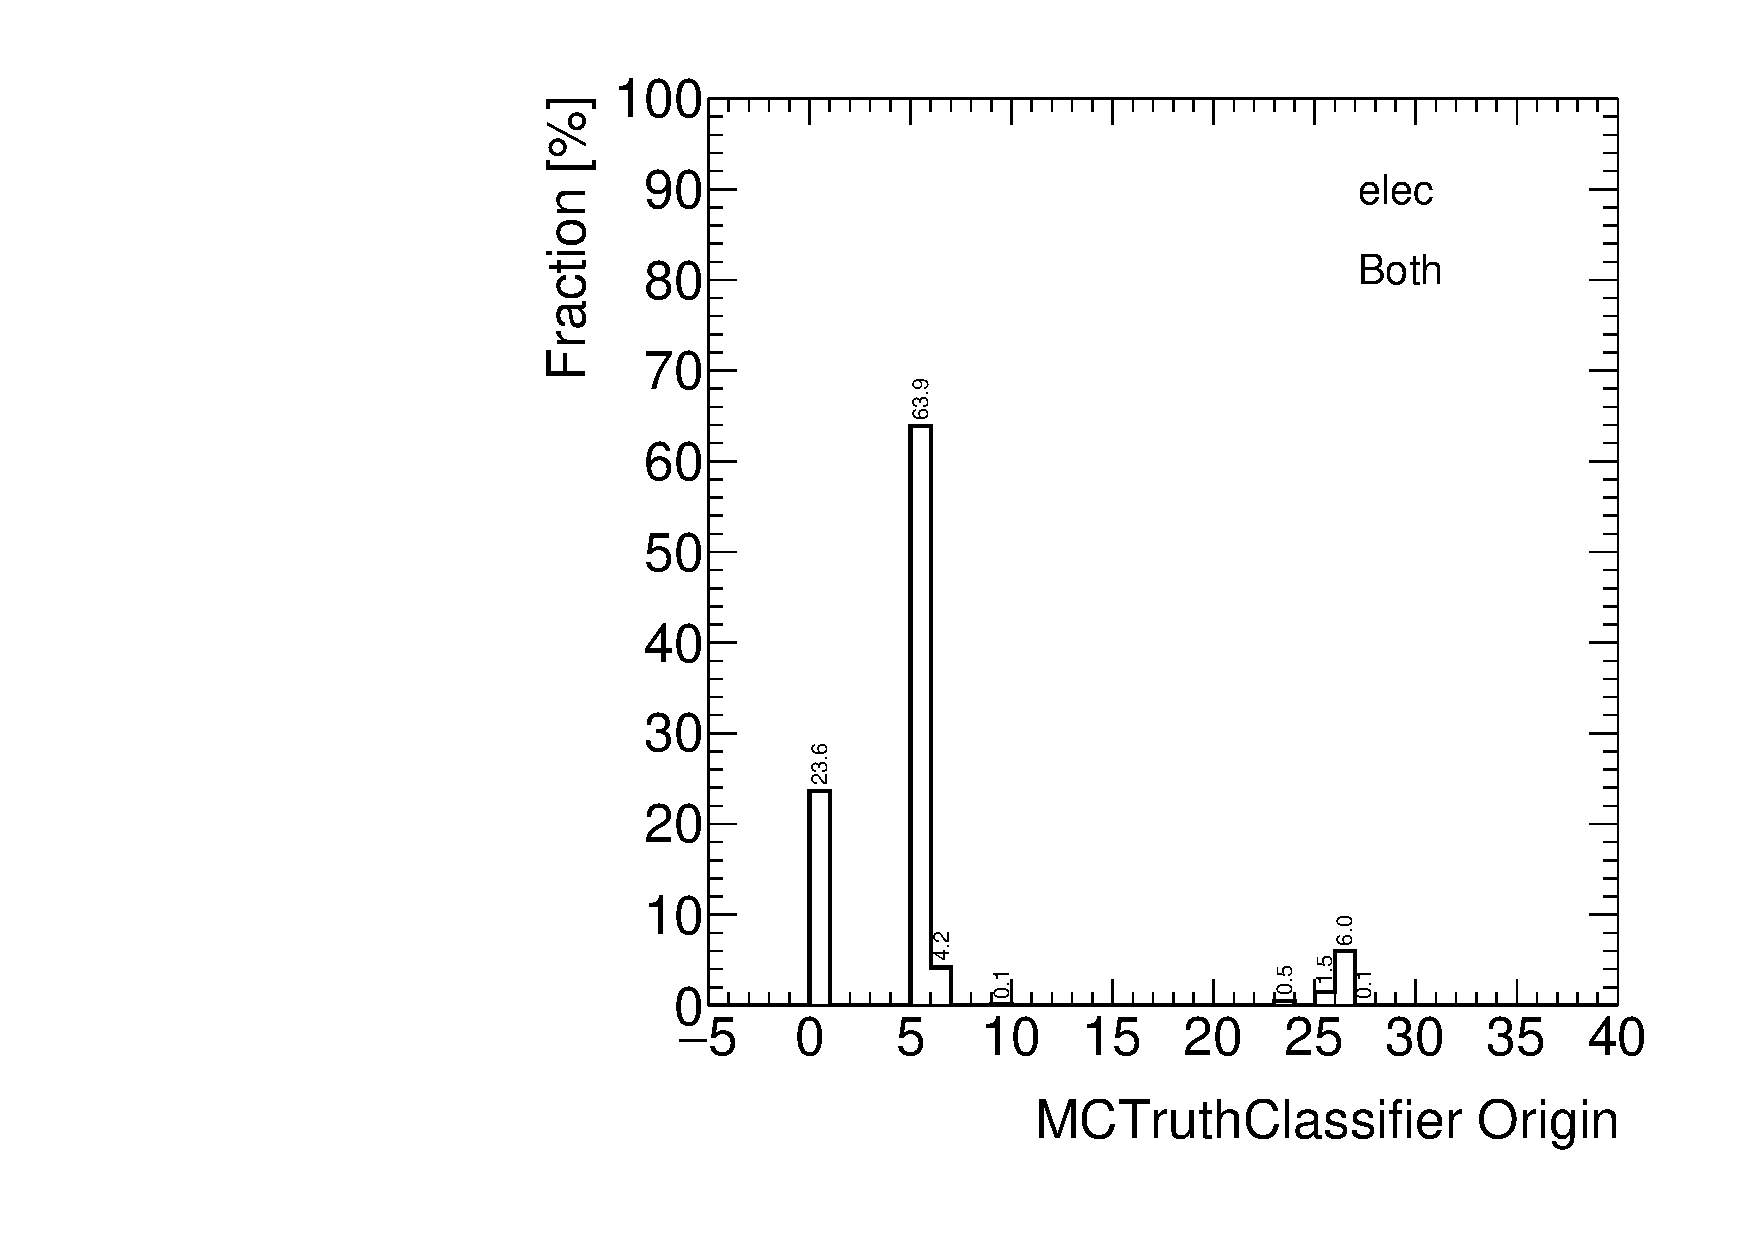
\includegraphics[scale=0.33]{./figures/boosted/FakeLeptons/JZXW_Origin_elec_Both}
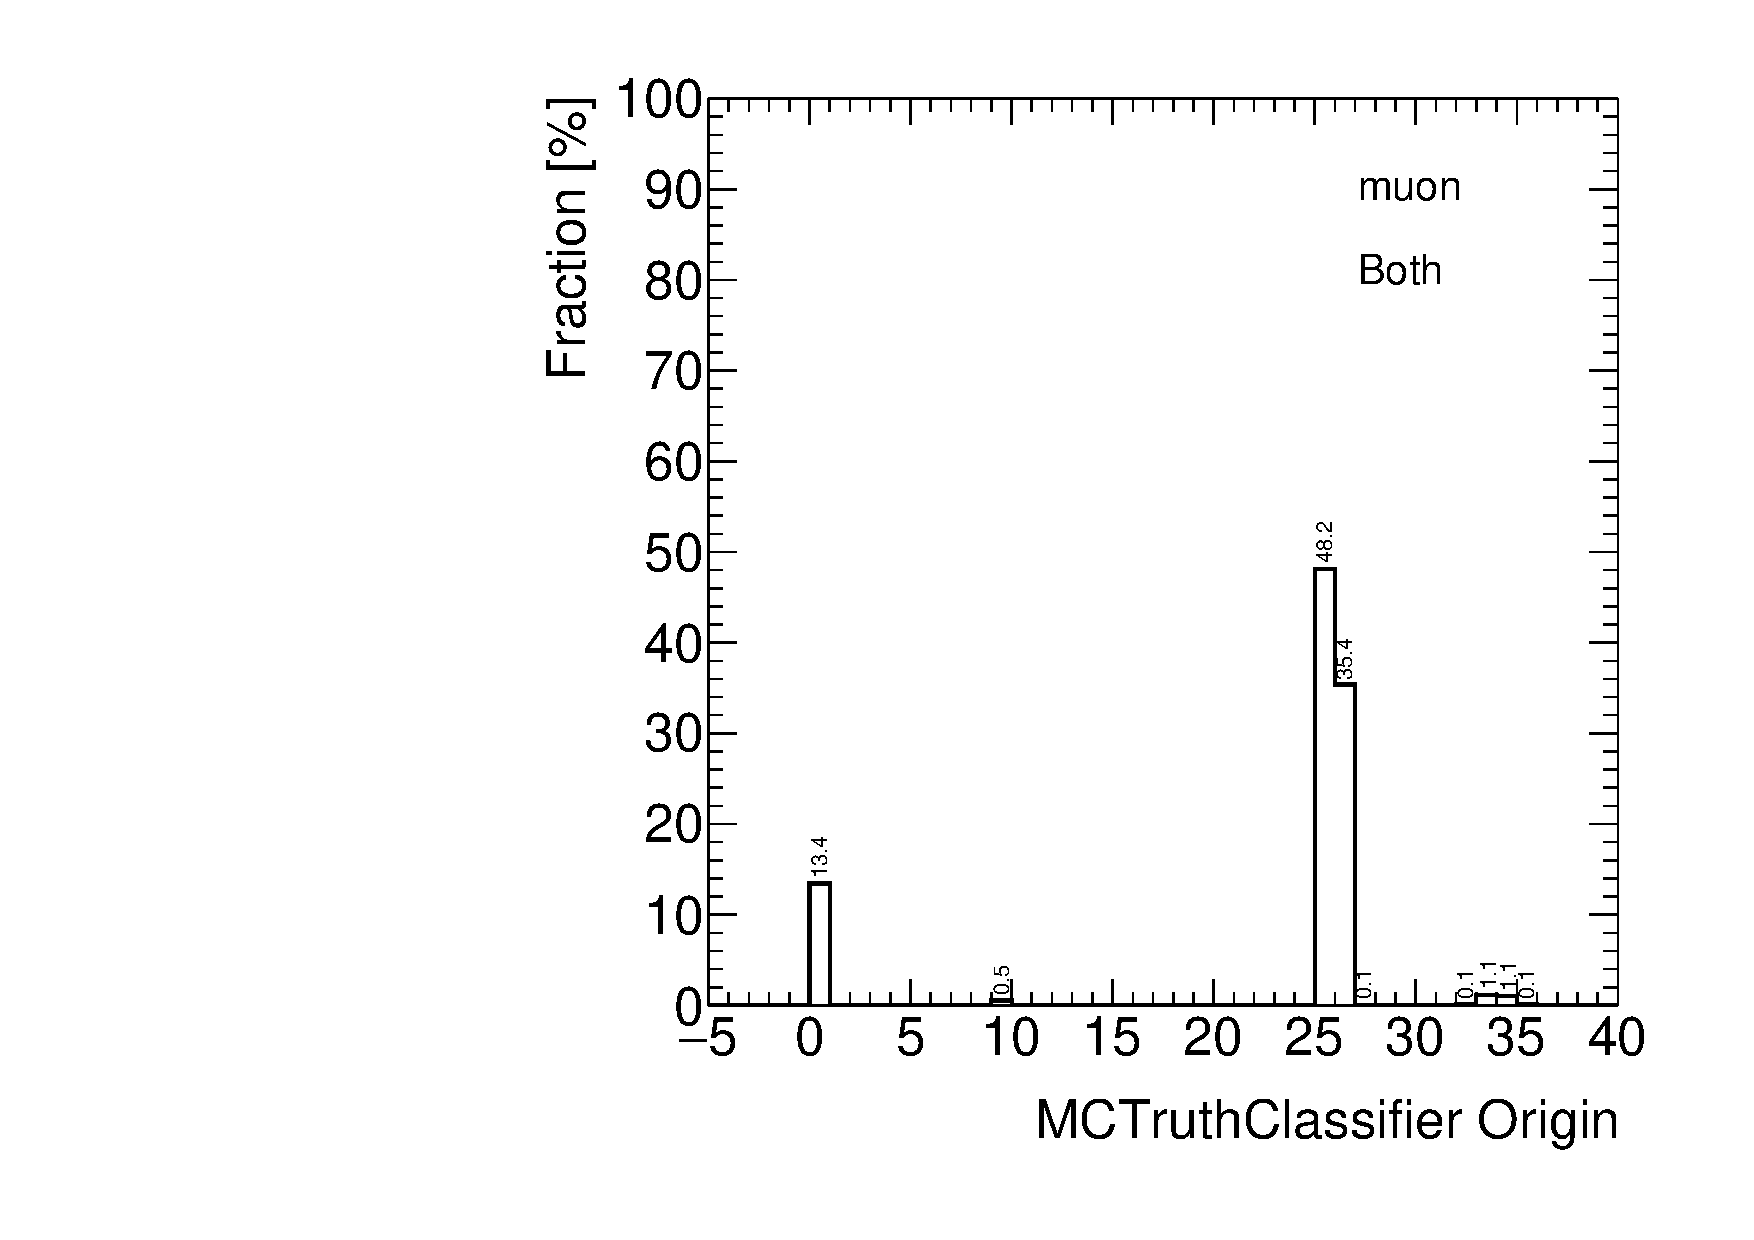
\includegraphics[scale=0.33]{./figures/boosted/FakeLeptons/JZXW_Origin_muon_Both}
\caption{Fraction of leptons from different origins. \textbf{No selection} on the reconstructed lepton $|d_{0}^{\textrm{sig}}|$ is applied.}
\label{fig:boosted_fakeorigin_nocut}
\end{center}
\end{figure}
\begin{figure}[!htbp]
\begin{center}
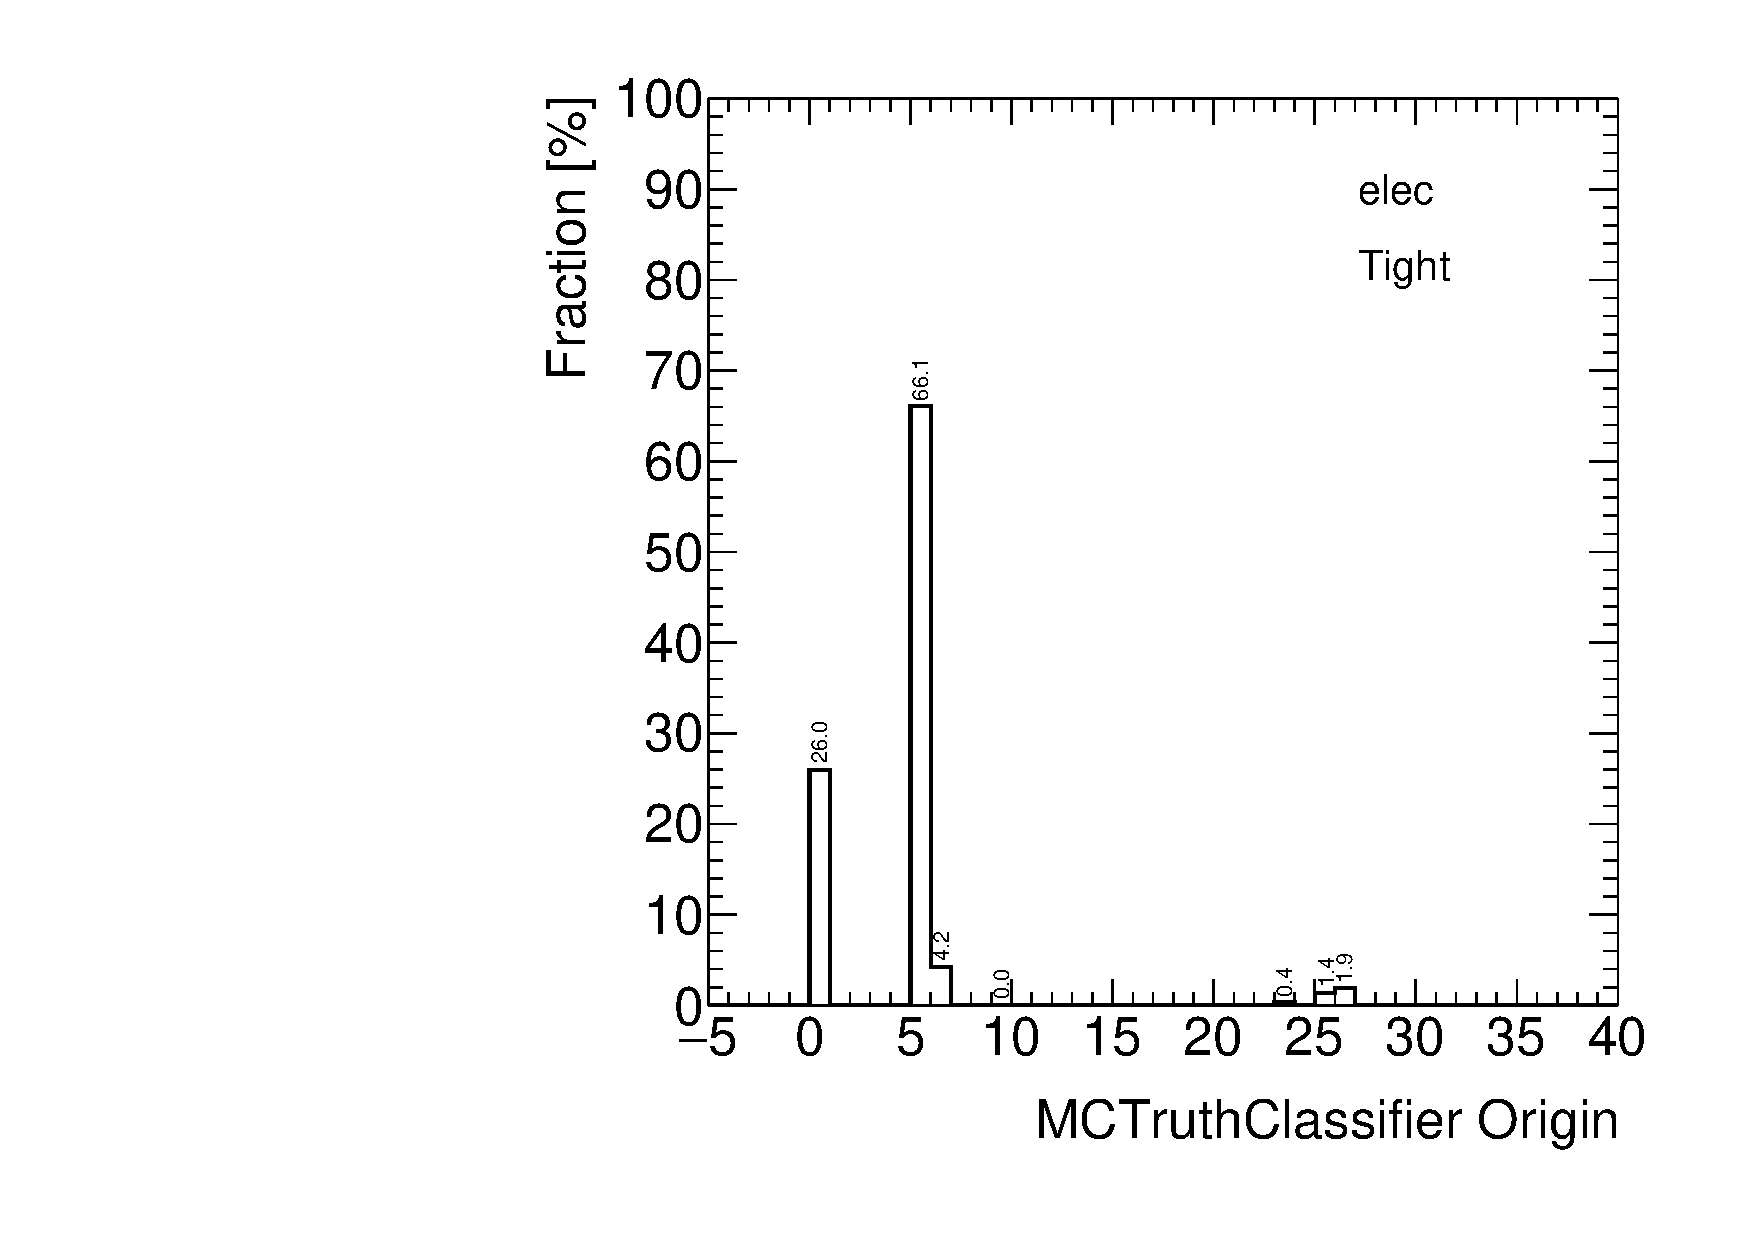
\includegraphics[scale=0.33]{./figures/boosted/FakeLeptons/JZXW_Origin_elec_Tight}
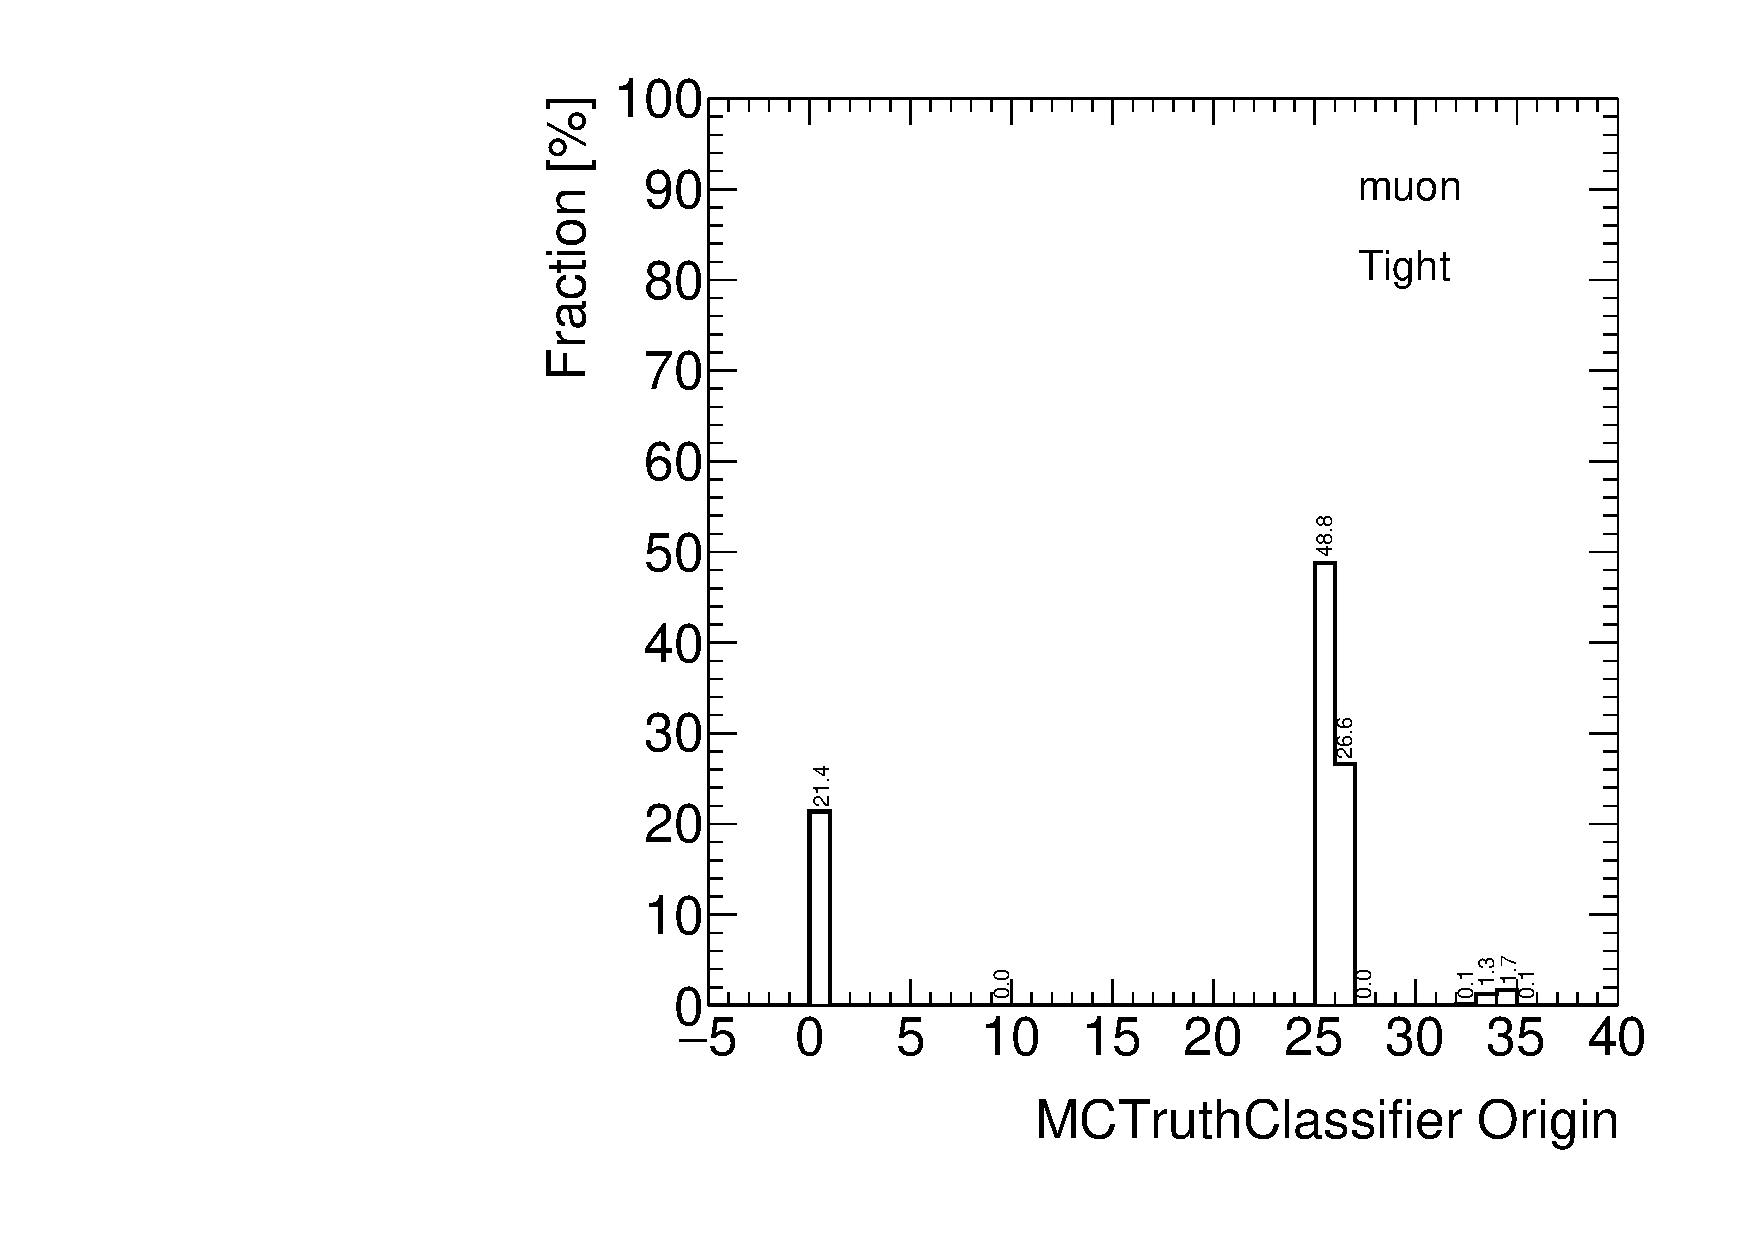
\includegraphics[scale=0.33]{./figures/boosted/FakeLeptons/JZXW_Origin_muon_Tight}
\caption{Fraction of leptons from different origins. Reconstructed leptons are required to \textbf{pass} the $|d_{0}^{\textrm{sig}}|$ < 2.0 selection.}
\label{fig:boosted_fakeorigin_passcut}
\end{center}
\end{figure}
\begin{figure}[!htbp]
\begin{center}
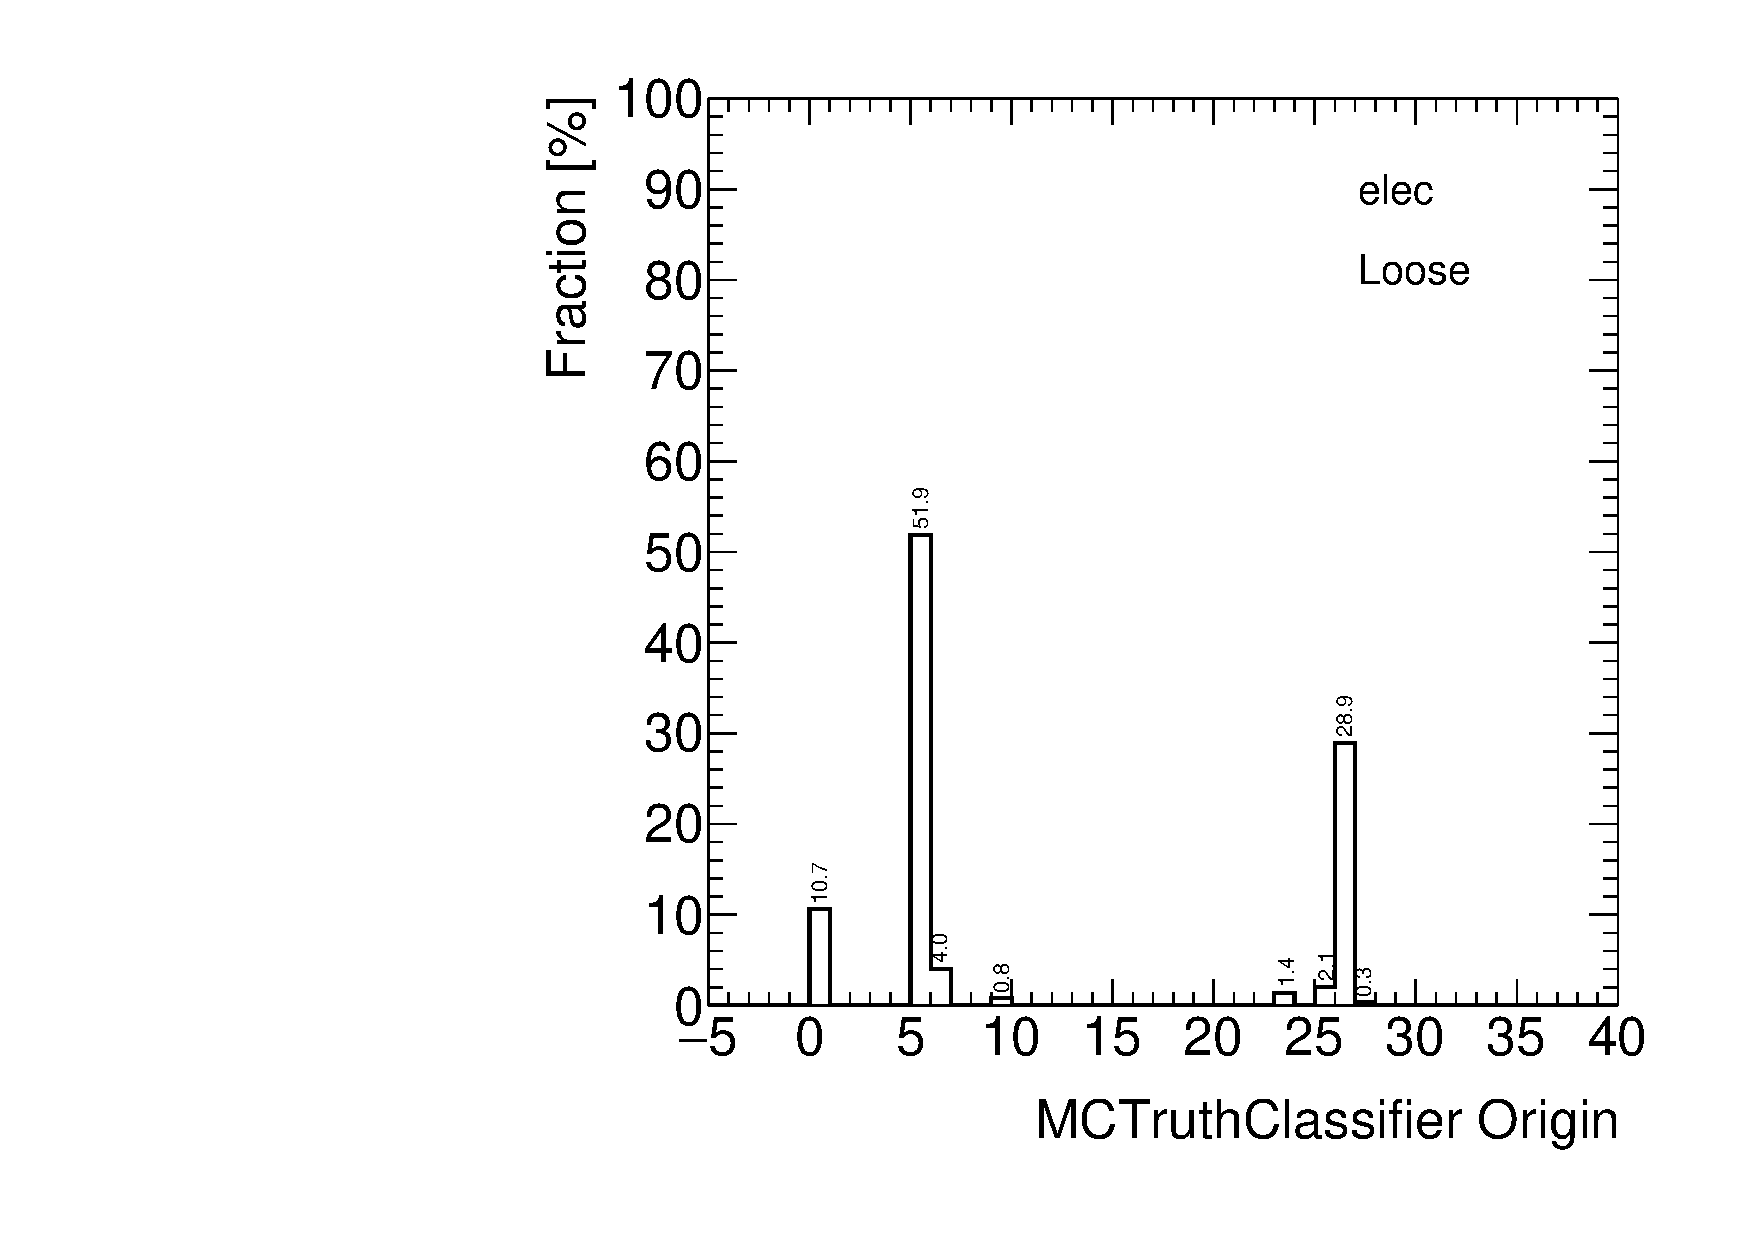
\includegraphics[scale=0.33]{./figures/boosted/FakeLeptons/JZXW_Origin_elec_Loose}
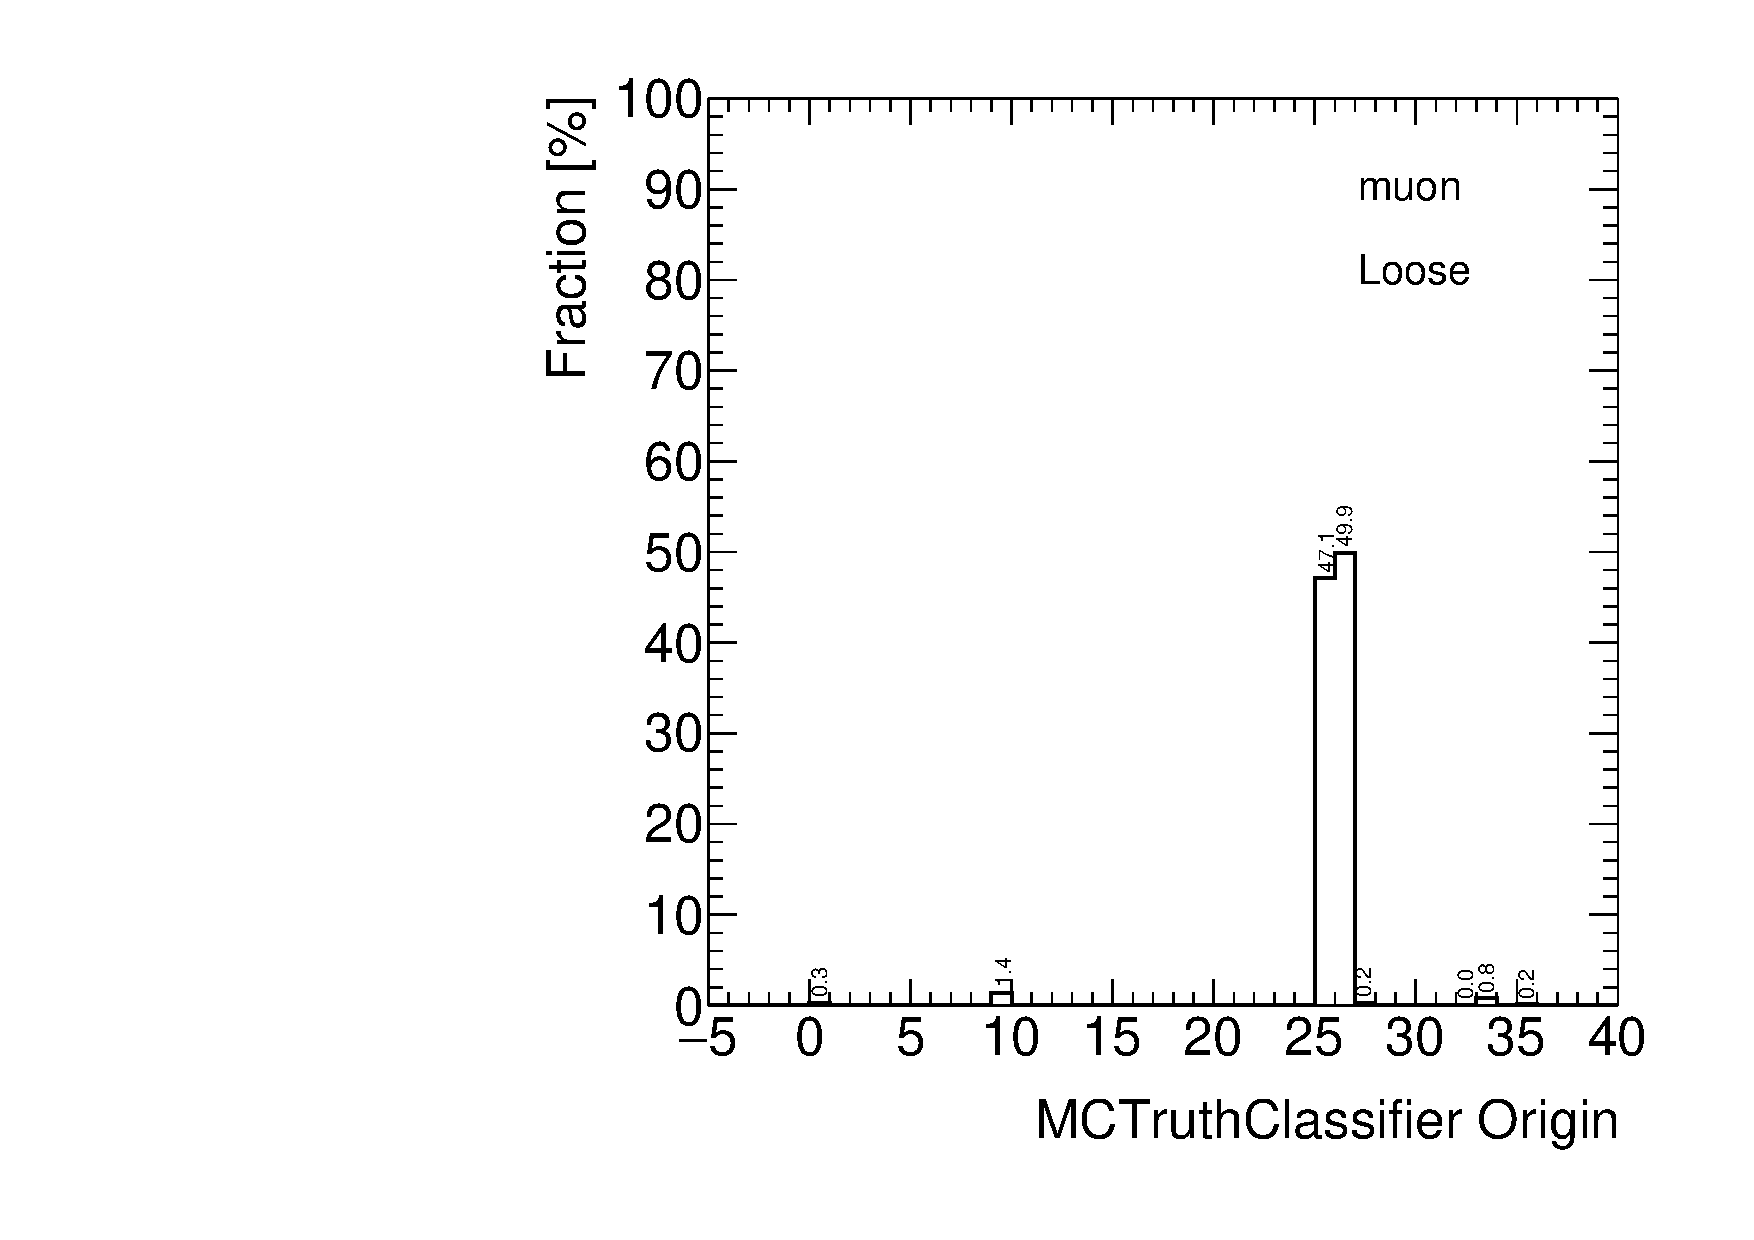
\includegraphics[scale=0.33]{./figures/boosted/FakeLeptons/JZXW_Origin_muon_Loose}
\caption{Fraction of leptons from different origins. Reconstructed leptons are required to \textbf{fail} the $|d_{0}^{\textrm{sig}}|$ < 2.0 selection.}
\label{fig:boosted_fakeorigin_loosecut}
\end{center}
\end{figure}








